\documentclass[11pt, oneside]{article}   	% use "amsart" instead of "article" for AMSLaTeX format
\usepackage{geometry}                		% See geometry.pdf to learn the layout options. There are lots.
\geometry{letterpaper}                   		% ... or a4paper or a5paper or ... 
%\geometry{landscape}                		% Activate for for rotated page geometry
%\usepackage[parfill]{parskip}    		% Activate to begin paragraphs with an empty line rather than an indent
\usepackage{graphicx}				% Use pdf, png, jpg, or eps� with pdflatex; use eps in DVI mode
								% TeX will automatically convert eps --> pdf in pdflatex		
\usepackage{amssymb}
\usepackage{amsmath}
\usepackage{parskip}
\usepackage{color}

\title{Poisson Distribution}
%\author{The Author}
%\section{}
% \subsection*{R code}
\date{}							% Activate to display a given date or no date

\graphicspath{{/Users/telliott_admin/Dropbox/Tex/png/}}

% \begin{center} 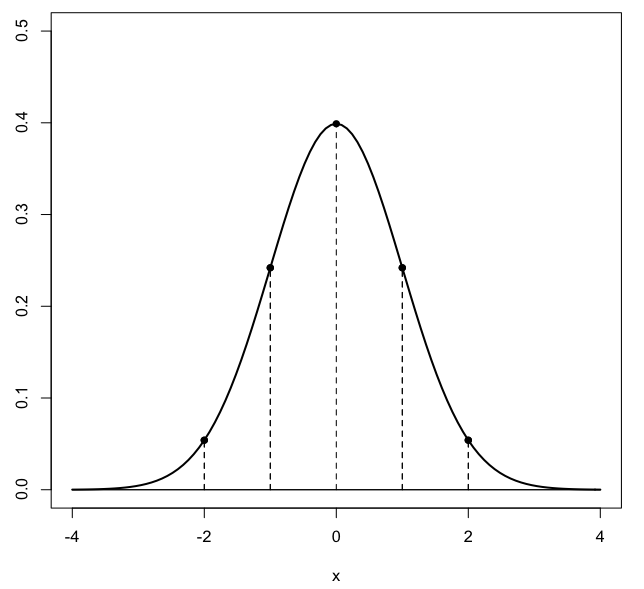
\includegraphics [scale=0.4] {gauss3.png} \end{center}
% \begin{bmatrix} a  &  b \\ c  &  d \end{bmatrix}
% \bigg |_

\begin{document}
\maketitle
\Large
%\noindent

The Poisson distribution is a special case of the binomial distribution for Bernoulli trials.  It is an approximation for situations in which the probability of success $p$ on each trial is small, and the number of trials $n$ is large, so that the mean $\lambda = np$ of successes is not too much greater than $1$ for the sequence of trials taken as a whole.

Recall that the binomial distribution for the number of successes $k$ on $n$ trials, with probability $p$ of success on each trial is:

\[ P(k) = {n\choose k} \  p^k \  (1-p)^{n-k} \]

where

\[ {n\choose k} =  \frac{n!}{k!  \ (n-k)!}  \]

Briefly, the derivation of this formula is that in independent trials with probability of success $p$ and of failure $q$, for a particular series of successes and failures, say:

\[ \textbf{S\ S\ F\ S\ S\ F\ F\ F\ F\ S\ S\ F\ F} \]

the probability is

\[ P = p \ p \ q \ p \ p \ q \ q \ q \ q \ p \ p \ q \ q = p^6 q^7 \]

and more generally, for $k$ successes in $n$ trials

\[ P = p^k q^{n-k} \]

Since $q = 1-p$

\[ = p^k (1-p)^{n-k} \]

The factor of
\[ \frac{n!}{ k! \ (n-k)! } \] 

counts the occurrence of the combinations, that is, all the permutations of 

\[ \textbf{SSFSSFFFFSSFF} \]
such as 

\[ \textbf{SSSSSSFFFFFFF} \]

 that have the \emph{same} number of total successes.

\subsection*{Simplifying ${n\choose k}$}

The first step involves the "choose" or combinations term. We are interested in problems where $n$ is large and $p$ is small, so that the mean number of successes is roughly near 1.  For $k=2$

\[ {n\choose 2} =  \frac{n!}{k!  \ (n-k)!}  \]
\[ = \frac{ n (n-1)}{k!} \ \frac{(n-2) (n-3) \cdots}{(n-2) (n-3) \cdots} \]
\[ = \frac{ n (n-1) }{ k! } \]
Since $n$ is large
\[  {n\choose 2} = \frac{ n (n-1) }{ k! } \approx \frac{n^2}{2!} \]

and more generally

\[ {n\choose k} \approx \frac{n^k}{k!}  \]

\subsection*{part 2}

The other term we will modify is

\[ (1-p)^{n-k} \]
\[ = \frac{(1-p)^n}{(1-p)^{k}} \]

The probability $p$ is quite small, but because $n$ is very large, we cannot just set $1-p$ equal to $1$ for the first term.

In contrast, $k$ is a modest size (say, $k < 10$) so we can reasonably set $1-p = 1$ for the second term, and thus the denominator is equal to $1$. The first term contributes much more than the second to the value for this expression.

Finally, we will show that $(1-p)^n \approx e^{-np}$.

Recall that

\[ e^x = 1 + x + \frac{x^2}{2!} + \cdots \approx 1 + x \]
(for small $x$)

Since $|p|$ is small, we have

\[ e^{-p} \approx 1 - p \]

so

\[ (1-p)^n \approx (e^{-p})^n = e^{-np} \]

Alternatively, we note that the binomial expansion (for $x$ near zero) is 
\[ (1 + x)^n \approx 1 + x \]
by a Taylor series.  Since both $(1-p)^n$ and $e^{-p}$ are approximately equal to $1-p$ they are approximately equal to each other.

\subsection*{Finishing up}

Substituting, we get

\[ P(k) = {n\choose k} \  p^k \  (1-p)^{n-k} \]
\[ \approx \frac{n^k}{k!} \ p^k \ e^{-np} \]

Introduce a symbol for the mean, $\lambda = np$

\[ P(k) \approx \frac{n^k}{k!} \ p^k \ e^{-\lambda} \]
\[ \approx  \frac{\lambda^k}{k!} \ e^{-\lambda} \]

This is the Poisson distribution for the number of successes $k$ in $n$ Bernoulli trials where the mean number of successes $np = \lambda$ over the whole series of trials is small.

\subsection*{The Poisson is normalized}

The Poisson distribution is normalized, i.e. it sums to $1$, and so is a real probability distribution.

\[ \sum\limits_{k=0}^{\infty} \frac{\lambda^k}{k!} \ e^{-\lambda} = e^{-\lambda} \ \sum\limits_{k=0}^{\infty} \frac{\lambda^k}{k!} = 1 \]

since

\[ \sum\limits_{k=0}^{\infty} \frac{{\lambda}^k}{k!} = \frac{{\lambda}^0}{0!} + \frac{{\lambda}^1}{1!} + \frac{{\lambda}^2}{2!} + \cdots  = e^{\lambda} \]


\subsection*{Note in passing}

I've always used different symbols (perhaps from Freifelder), although the ones shown above are standard in statistics.  In my preferred notation the mean is $m$ and the number of successes is $i$ so the equation is

\[ P(i) = \frac{e^{-m} \ m^i }{ i! } \]

which I remember as "Emmy!" or more explicitly, "emmii!".

One useful thing to remember about the Poisson distribution is that it always simplifies dramatically for $P(0)$, and sometimes for $P(1)$.

\[ P(i) = \frac{e^{-m} \ m^i }{ i! } \]
\[ P(0) = \frac{e^{-m} \ m^0 }{ 0! } \]
\[ P(0) = e^{-m} \]

When the mean is one, $m = 1$

\[ P(0) = \frac{1}{e} \]
\[ \approx 0.368 \]

and 

\[ P(1) = \frac{e^{-1} \ 1^1 }{ 1! } = \frac{1}{e} \]

For example, if we take a box that is divided into one hundred compartments and throw one hundred marbles into it randomly, then at the end of the experiment slightly more than $1/3$ of the compartments will still be empty, an equal number will contain one marble, and about 25 percent will contain more than $1$.

The same holds for a bacterial culture infected with virus at a ratio of one virus per bacterial cell.  At an $ moi = 1$ ("m.o.i." is short for "multiplicity of infection"), more than one-third of the cells will be uninfected.

Here is a plot of the Poisson distribution for various values of $\lambda$ ($m$).

\begin{center} 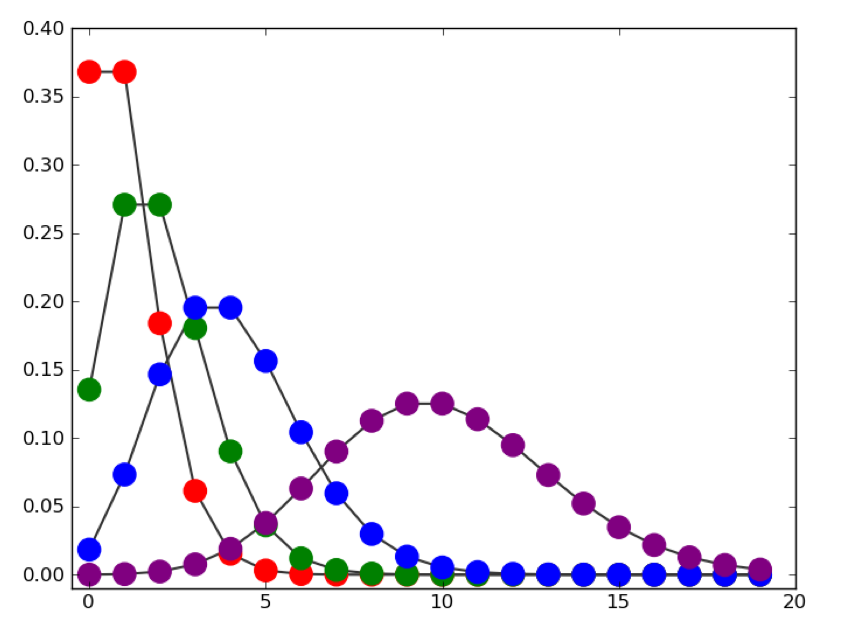
\includegraphics [scale=0.4] {poisson.png} \end{center}

Note the very small values for $P > 10$ when $m < 5$ (red, green, and blue).  That's the inverse factorial talking.

\subsection*{Genetics}

One application is to bacterial genetics.  Consider the Luria-Delbruck experiment, in which mutant bacteria resistant to the action of the bacterial virus T1 were selected.  A modern (Darwinian) view appreciates that the mutations which confer virus-resistance pre-exist in the population, having occurred randomly during growth.  

An alternative, the Lamarckian view, suggests that the mutations arise \emph{in response} to each bacterium's encounter with the virus.

So if we have an agar plate whose surface contains $10^8$ bacterial cells and an excess of virus particles, we can model the Lamarckian view as a process in which each cell has an extremely small probability of surviving the phage assault, but the large number of cells constitutes a large number of trials.  We adjust the mean number of successes (phage-resistant colonies per plate) to be near $1$.  Then, the Poisson approximation should apply.

In particular, if $f$ is the fraction of plates which have no resistant colonies, then in

\[ P(i=0) = \frac{e^{-m} \ m^i }{ i! } \]

both $m^i$ and $i!$ equal $1$ and so

\[ P(i=0) = f = e^{-m} \]
\[ m = - \ln f \]

For example, if $f=0.5$, then $m=0.69$.  Now we can calculate $P(i=1)$, $P(i=2)$, and the whole distribution.  Here is the probability distribution for $m=1$ and $i=0 \cdots 5$:

\[
\begin{matrix}
0 & 0.368 \\
1 & 0.368 \\
2 & 0.184 \\
3 & 0.061 \\
4 & 0.015 \\
5 & 0.003 \\
\end{matrix}
\]

and here is the cumulative distribution:

\[
\begin{matrix}
0 & 0.368 \\
1 & 0.736 \\
2 & 0.92 \\
3 & 0.981 \\
4 & 0.996 \\
5 & 0.999 \\
\end{matrix}
\]

The probability of observing 6 or more colonies is less than $1/1000$.

Crucially, this is \emph{not} what one observes.  Instead, jackpots containing dozens or even hundreds of colonies are obtained at a frequency of about 1 plate in 10.  

In summary, the results are inconsistent with the Lamarckian view, but are easily explained by a model where mutations occur randomly with respect to each cell division.  If a mutation happens to occur early in the growth of a culture, that mutant cell will have a large number of descendants, each of which can form a phage-resistant colony.

\end{document}  